%------------------------------------------------------------------------------
% Author(s):
% Varaun Ramgoolie
%
% Copyright:
%  Copyright (C) 2020 Brad Bachu, Arjun Mohammed, Varaun Ramgoolie, Nicholas Sammy
%
%  This file is part of Applied-Mathematics-Unit2 and is distributed under the
%  terms of the MIT License. See the LICENSE file for details.
%
%  Description:
%     Year: 2008 June
%     Module: 3
%     Question: 6
%------------------------------------------------------------------------------

%------------------------------------------------------------------------------
% 6 a
%------------------------------------------------------------------------------

We are given two particles which are launched at different angles to the horizontal.

\begin{subquestions}
	
\subquestion

\textbf{\textit{Sketch and Translate:}} \\ \\
\begin{figure}[H]
	\begin{center}
		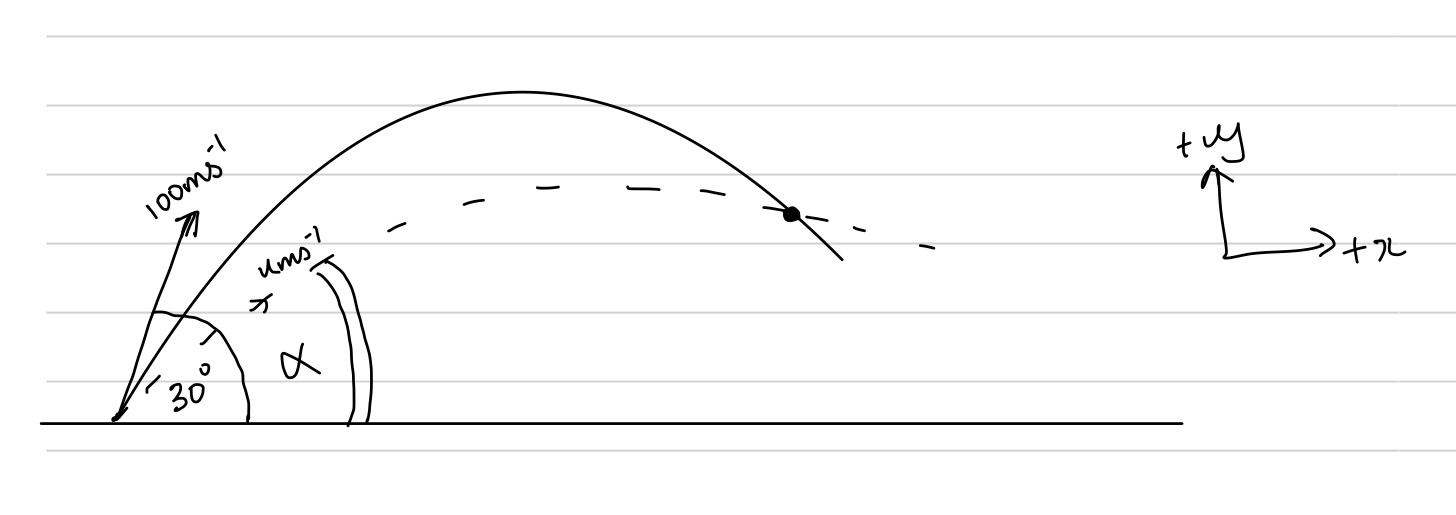
\includegraphics[scale=0.25]{../2008/figures/2008Jq6-1}
		\caption{\label{2008J:q6:Sketch1} Projectiles launched from fixed point.}
	\end{center}
\end{figure}
At the greatest height, the vertical velocity of the first particle, $V_y$, is 0.




\textbf{\textit{Simplify and Diagram:}} \\ \\
\begin{figure}[H]
	\begin{center}
		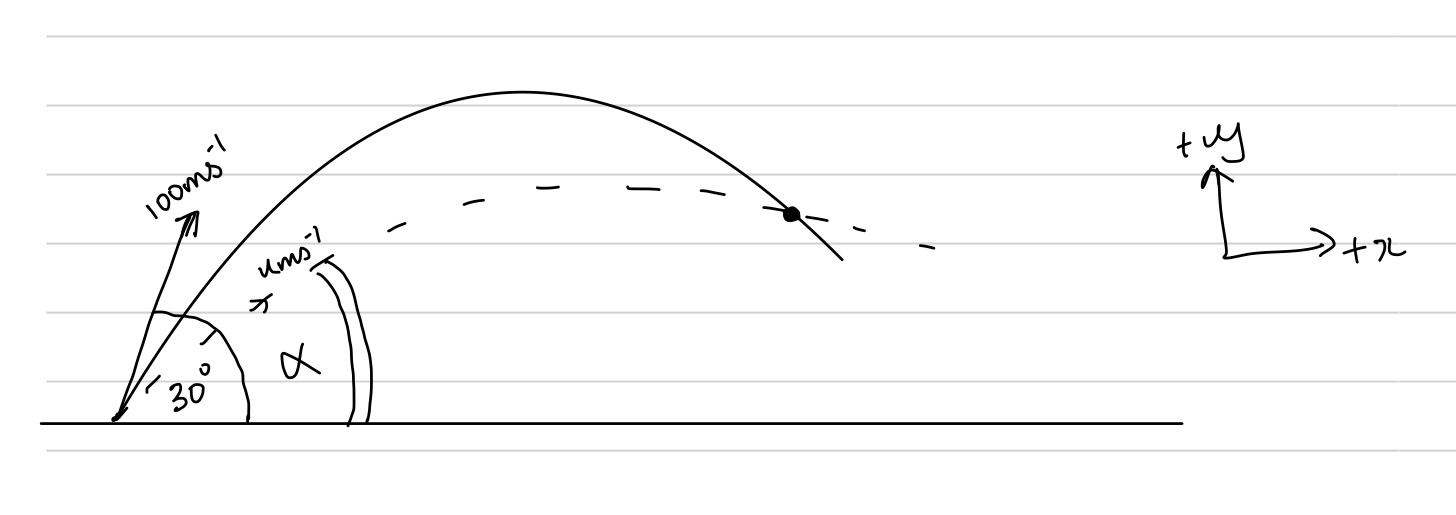
\includegraphics[scale=0.25]{../2008/figures/2008Jq6-1}
		\caption{\label{2008J:q6:Diagram1} Projectiles launched from fixed point.}
	\end{center}
\end{figure}
We can resolve the motion of the first particle in the vertical ($y$) and horizontal ($x$) directions and then use our equations of motion to solve for the greatest height reached by the first particle.




\textbf{\textit{Represent Mathematically:}} \\ \\
By resolving the motion of the first particle, we get that,
\begin{align}
	U_x & = 100 \cos(30) \,, \nn \\
	A_x & = 0 \,, \nn \\
	U_y & = 100 \sin(30) \,, \nn \\
	A_y & = -10 \,. 
\end{align}
where $U_x$ and $A_x$ are the horizontal initial velocity and acceleration and similarly $U_y$ and $A_y$ are the vertical initial velocity and acceleration.

At the greatest height, we get that,
\begin{equation}
	V_y = 0 \,.
\end{equation}
where $V_y$ is the final vertical velocity of the first particle.

The equation that we will use to find the greatest height is,
\begin{align}
	V_y^2 & = U_y^2 + 2A_yS_y \nn \\
	\implies S_y & = \frac{V_y^2-U_y^2}{2a_y} \label{2008J:q6:SEqn1} \,.
\end{align}




\textbf{\textit{Solve and Evaluate:}} \\ \\
Using \req{2008J:q6:SEqn1}, we get that,
\begin{align}
	S_y & = \frac{0^2-(100\sin(30))^2}{2(-10)} \nn \\
		& = 125m \,.
\end{align}

%------------------------------------------------------------------------------
% 6 b
%------------------------------------------------------------------------------

\subquestion

\begin{subsubquestions}
	
\subsubquestion

\textbf{\textit{Simplify and Diagram:}} \\ \\
We can consider \rfig{2008J:q6:Diagram1}. We will use our equations of motion with $t=5$.




\textbf{\textit{Represent Mathematically:}} \\ \\			
The equation that we will use to find the horizontal distance is,
\begin{equation}
	S_x =U_xt + \frac{1}{2}A_xt^2 \,.	
\end{equation}




\textbf{\textit{Solve and Evaluate:}} \\ \\
The horizontal distance traveled by the first particle after 5s is,
\begin{align}
	S_x & = 100\cos(30)(5) + \frac{1}{2}(0)5^2 \nn \\
	    & = 250\sqrt{3}m \,.
\end{align}

%------------------------------------------------------------------------------

\subsubquestion

\textbf{\textit{Represent Mathematically:}} \\ \\			
The equation that we will use to find the vertical distance is,
\begin{equation}
	S_y =U_yt + \frac{1}{2}A_yt^2 \,.	
\end{equation}




\textbf{\textit{Solve and Evaluate:}} \\ \\
The vertical distance traveled by the first particle after 5s is,
\begin{align}
	S_y & = 100\sin(30)(5) + \frac{1}{2}(-10)5^2 \nn \\
		& = 125m \,.
\end{align}

%------------------------------------------------------------------------------

\subsubquestion

\textbf{\textit{Simplify and Diagram:}} \\ \\
We can still consider \rfig{2008J:q6:Diagram1}. We should notice that, from the setup of the question, the position of the second particle after $t=4s$ will have the same corresponding values as (b)(i) and (b)(ii) as we are given that the second particle hits the first particle after being launched 1 second later. To find the values of the expressions for the question, we will resolve the initial velocity in the $x$ and $y$ directions and use our equations of motion.




\textbf{\textit{Represent Mathematically:}} \\ \\
The initial velocity is resolved as,
\begin{align}
	u_x & = u\cos(\alpha) \,, \nn \\
	a_x & = 0 \,, \nn \\
	u_y & = u\sin(\alpha) \,, \nn \\
	a_y & = -10 \,.
\end{align}

To solve this problem, we will use,
\begin{equation}
	s_x = u_xt + \frac{1}{2}a_xt^2 \,.
\end{equation}




\textbf{\textit{Solve and Evaluate:}} \\ \\
At $t=4$, we substitute the values $s_x=S_x=250\sqrt{3}$ and $a_x=0$ to get that,
\begin{align}
	250\sqrt{3} & = u_x(4) + \frac{1}{2}(0)(4)^2 \nn \\
	\implies u_x & = u\cos(\alpha) = \frac{125\sqrt{3}}{2}ms^{-1} \,.
\end{align} 

%------------------------------------------------------------------------------

\subsubquestion

\textbf{\textit{Represent Mathematically:}} \\ \\
To solve this problem, we will use,
\begin{equation}
	s_y = u_yt + \frac{1}{2}a_yt^2 \,.
\end{equation}




\textbf{\textit{Solve and Evaluate:}} \\ \\
At $t=4$, we substitute the values $s_y=S_y=125$ and $a_y=-10$ to get that,
\begin{align}
	125 & = u_y(4) + \frac{1}{2}(-10)(16) \nn \\
	u_y & = u\sin(\alpha) = \frac{205}{4}ms^{-1} \,.
\end{align}

%------------------------------------------------------------------------------

\subsubquestion

\textbf{\textit{Solve and Evaluate:}} \\ \\
To find $u$, we can use,
\begin{align}
	(u\sin(\alpha))^2 + (u\cos(\alpha))^2 & = \left(\frac{205}{4}\right)^2 + \left(\frac{125\sqrt{3}}{2}\right)^2 \nn \\
	 u^2\left(\sin^2(\alpha)+\cos^2(\alpha)\right) & = \left(\frac{205}{4}\right)^2 + \left(\frac{125\sqrt{3}}{2}\right)^2 \nn \\
	 \implies u & = \sqrt{\left(\frac{205}{4}\right)^2 + \left(\frac{125\sqrt{3}}{2}\right)^2} \nn \\
	            & = 119.8ms^{-1}
\end{align}

%------------------------------------------------------------------------------

\subsubquestion

\textbf{\textit{Solve and Evaluate:}} \\ \\
To find $\alpha$, we can use,
\begin{align}
	\frac{u\sin(\alpha)}{u\cos(\alpha)} & = \frac{\frac{205}{4}}{\frac{125\sqrt{3}}{2}} \nn \\
	\tan(\alpha) & = \frac{41}{50\sqrt{3}} \nn \\
	\implies \alpha & = \arctan\left(\frac{41}{50\sqrt{3}}\right) = 25.3^o \,.
\end{align}
	
\end{subsubquestions}

\end{subquestions}
	